\newpage
\subsection{CAD Model}
In order to digitally design add-ons for the SplashDrone 4, the drone has to be modelled using computer-aided design software. To save time, close-range photogrammetry was used to capture the base of the drone.

Photogrammetry can be described as extracting \gls{3D} information from photographs. The process involves taking overlapping photographs of an object and converting them into \gls{3D} digital models, stitching the images together. 163 high resolution photographs were taken with a DJI Osmo Pocket \cite{osmopocket}, resulting in a raw dataset of 933\gls{MiB}. The dataset is available on GitHub \cite{dronemodel}. Autodesk ReCap Photo was used for the conversion into a \gls{CAD} Model \cite{autodeskrecap}

To get the best results, several requirements must be met. Creative ways were found to pass these requirements when capturing the drone at home:

\begin{center}
\begin{tabular}{ |c|c| } 
 \hline
 Requirement & Fix  \\ 
 \hline
 Object must have texture & Smear removable shoe polish on the body \\ 
 Object must not be reflective & Mask the reflective dome with toilet paper \\ 
 Base must have variation & Use colourful bed sheets \\ 
 Lighting conditions must be consistent & Use a beach umbrella to diffuse the sun light \\ 
 \hline
\end{tabular}
\end{center}

Initial conversion seemed to be good, though some small patching had to be done, especially on the motors:

\begin{figure}[h]
  \centering
  \begin{minipage}[b]{0.4\textwidth}
    \includegraphics[width=\textwidth]{070_design/cadmodel/31_dphoto.jpg}
    \caption{Original photo \cite{dronemodel}}
  \end{minipage}
  \hfill
  \begin{minipage}[b]{0.5\textwidth}
    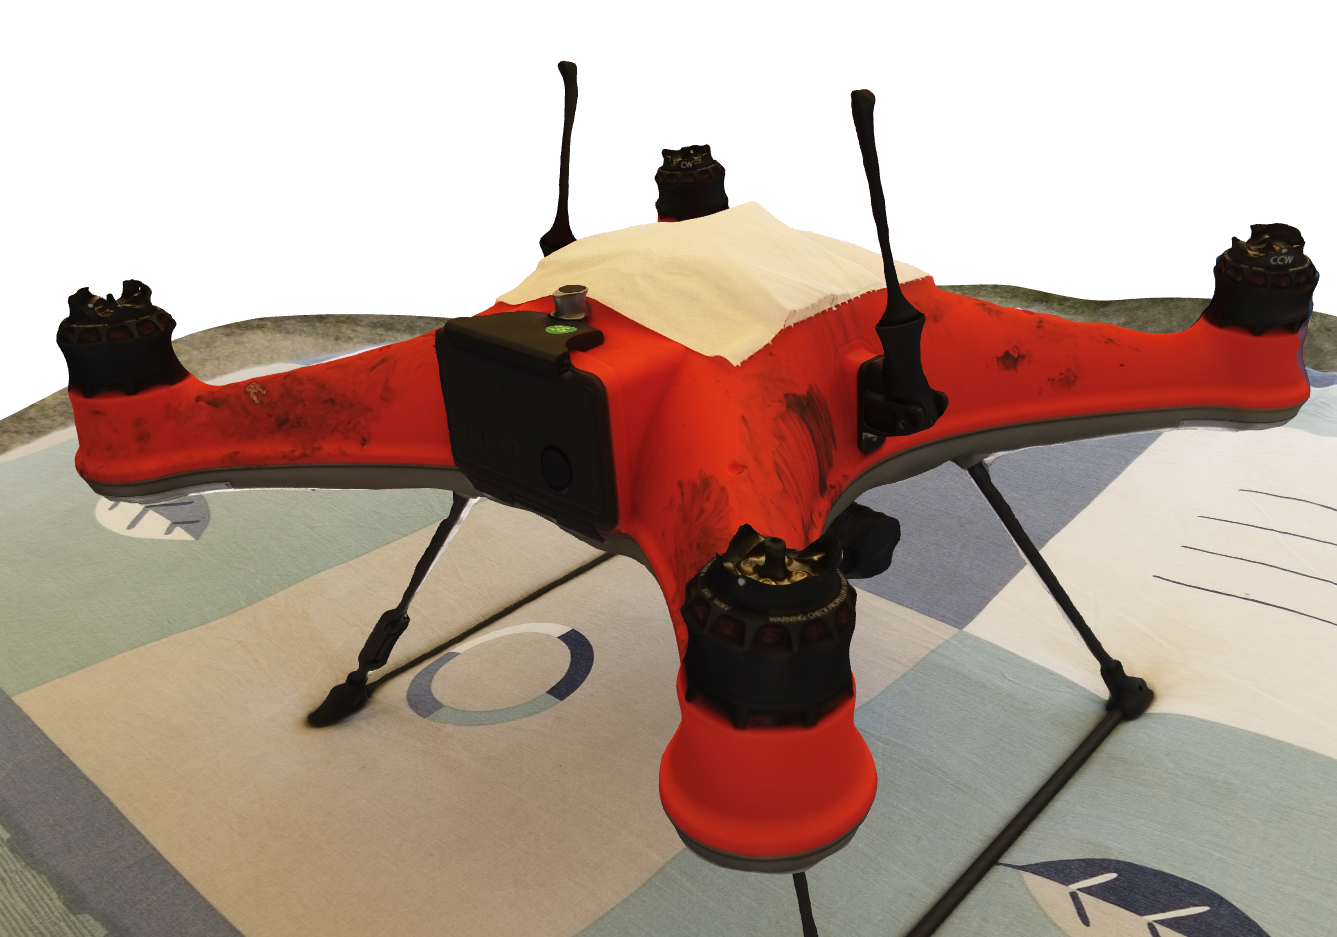
\includegraphics[width=\textwidth]{070_design/cadmodel/32_dmodel.png}
    \caption{3D Model \cite{dronemodel}}
  \end{minipage}
\end{figure}

The program failed to capture the gimbal of the drone accurately as it was able to move freely during capture. The bottom has been roughly reworked later on in \gls{CAD} software, leading to the following result:

\begin{figure}[h]
\centering
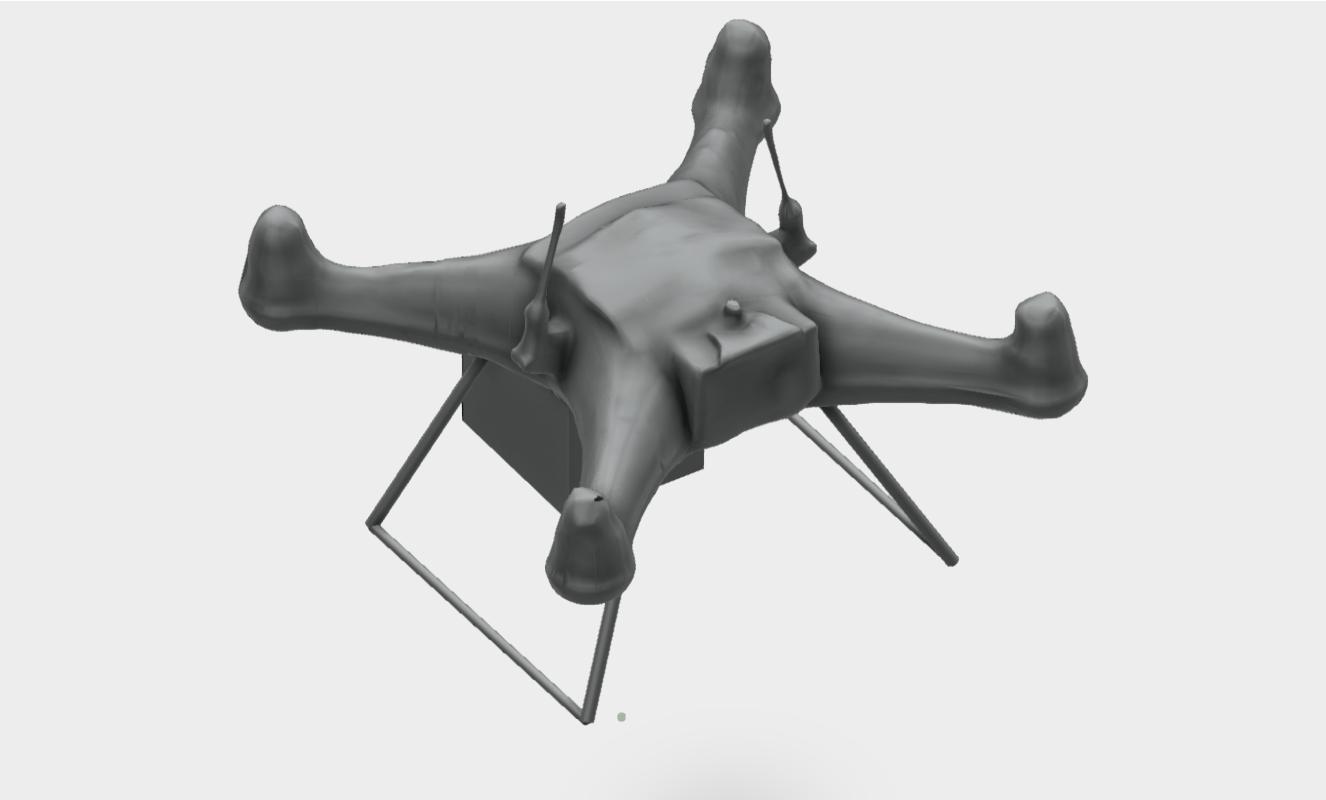
\includegraphics[scale=0.1]{070_design/cadmodel/33_dcadmodel.png}
\caption{Final CAD Model \cite{dronemodel}}
\end{figure}

As the gimbal of the drone is not of any importance, it is not modelled and instead modelled as a \gls{3D} box. While the model is not perfect, it is adequate for our use case.

